\documentclass[a4paper,14pt]{extreport}
  \usepackage[left=1.5cm,right=1.5cm,
      top=1.5cm,bottom=2cm,bindingoffset=0cm]{geometry}
  \usepackage{scrextend}
  \usepackage[T1,T2A]{fontenc}
  \usepackage[utf8]{inputenc}
  \usepackage[english,russian,ukrainian]{babel}
  \usepackage{tabularx}
  \usepackage{amssymb}
  \usepackage{color}
  \usepackage{amsmath}
  \usepackage{mathrsfs}
  \usepackage{listings}
  \usepackage{graphicx}
  \graphicspath{ {./images/} }
  \usepackage{lipsum}
  \usepackage{xcolor}
  \usepackage{hyperref}
  \usepackage{tcolorbox}
  \usepackage{tikz}
  \usepackage[framemethod=TikZ]{mdframed}
  \usepackage{wrapfig,boxedminipage,lipsum}
  \mdfdefinestyle{MyFrame}{%
  linecolor=blue,outerlinewidth=2pt,roundcorner=20pt,innertopmargin=\baselineskip,innerbottommargin=\baselineskip,innerrightmargin=20pt,innerleftmargin=20pt,backgroundcolor=gray!50!white}
   \usepackage{csvsimple}
   \usepackage{supertabular}
  \usepackage{pdflscape}
  \usepackage{fancyvrb}
  %\usepackage{comment}
  \usepackage{array,tabularx}
  \usepackage{colortbl}
   \usepackage{fp}

  \usepackage{varwidth}
  \tcbuselibrary{skins}
  \usepackage{fancybox}
  \usepackage{spreadtab}
   % Цвета для гиперссылок
  \definecolor{linkcolor}{HTML}{799B03} % цвет ссылок
  \definecolor{urlcolor}{HTML}{799B03} % цвет гиперссылок


  \usepackage{tikz}
  \usepackage[framemethod=TikZ]{mdframed}
  \usepackage{xcolor}
  \usetikzlibrary{calc}
  \makeatletter
  \newlength{\mylength}
  \xdef\CircleFactor{1.1}
  \setlength\mylength{\dimexpr\f@size pt}
  \newsavebox{\mybox}
  \newcommand*\circled[2][draw=blue]{\savebox\mybox{\vbox{\vphantom{WL1/}#1}}\setlength\mylength{\dimexpr\CircleFactor\dimexpr\ht\mybox+\dp\mybox\relax\relax}\tikzset{mystyle/.style={circle,#1,minimum height={\mylength}}}
  \tikz[baseline=(char.base)]
  \node[mystyle] (char) {#2};}
  \makeatother

  \definecolor{ggreen}{rgb}{0.4,1,0}
  \definecolor{rred}{rgb}{1,0.1,0.1}
  \definecolor{amber}{rgb}{1.0, 0.75, 0.0}
  \definecolor{babyblue}{rgb}{0.54, 0.81, 0.94}
  \definecolor{amethyst}{rgb}{0.6, 0.4, 0.8}

  \usepackage{float}
  \usepackage{wrapfig}
  \usepackage{framed}
  %for nice Code{
  \lstdefinestyle{customc}{
    belowcaptionskip=1\baselineskip,
    breaklines=true,
    frame=L,
    xleftmargin=\parindent,
    language=C,
    showstringspaces=false,
    basicstyle=\small\ttfamily,
    keywordstyle=\bfseries\color{green!40!black},
    commentstyle=\itshape\color{purple!40!black},
    identifierstyle=\color{blue},
    stringstyle=\color{orange},
  }
  \lstset{escapechar=@,style=customc}
%}


\begin{document}
  \pagecolor{white}

  %----------------------------------------1
  \newtcbox{\xmybox}[1][red]{on line, arc=7pt,colback=#1!10!white,colframe=#1!50!black, before upper={\rule[-3pt]{0pt}{10pt}},boxrule=1pt, boxsep=0pt,left=6pt,right=6pt,top=2pt,bottom=2pt}

  \begin{titlepage}
    \begin{center}
      \large
      Національний технічний університет України \\ "Київський політехнічний інститут імені Ігоря Сікорського"


      Факультет Електроніки

      Кафедра мікроелектроніки
      \vfill

      \textsc{ЗВІТ}\\

      {\Large Про виконання лабораторної роботи №4\\
        з дисципліни: «Фізичні основи сенсорики»\\[1cm]

          Електрохімічні сенсори


      }
    \bigskip
  \end{center}
  \vfill

  \newlength{\ML}
  \settowidth{\ML}{«\underline{\hspace{0.4cm}}» \underline{\hspace{2cm}}}
  \hfill
  \begin{minipage}{1\textwidth}
  Виконавець:\\
  Студент 4-го курсу \hspace{4cm} $\underset{\text{(підпис)}}{\underline{\hspace{0.2\textwidth}}}$  \hspace{1cm}А.\,С.~Мнацаканов\\
  \vspace{1cm}

  Перевірив: \hspace{6.1cm} $\underset{\text{(підпис)}}{\underline{\hspace{0.2\textwidth}}}$  \hspace{1cm}ас. Коваль В. М.\\

  \end{minipage}

  \vfill

  \begin{center}
  2021
  \end{center}
\end{titlepage}



\newpage
\setcounter{page}{2}
\textbf{Мета роботи} – дослідити процеси, що відбуваються в гальванічній
електрохімічній комірці з однорідним та неоднорідним електролітом.


\begin{center}
\textbf{Порядок виконання роботи}
\end{center}
\begin{enumerate}
  \item Помістити пару електродів з системи алюміній-мідних електродів в
  катодне та анодне відділення електрохімічної комірки з однорідним електролітом.
  \item За допомогою мікроамперметра М93 виміряти струм в електрохімічній
  комірці з однорідним електролітом для різних електродних пар: Cu-Cu, Al-Cu, Cu-
  Al.
  \item Помістити систему на основі графітових електродів в катодне та анодне
  відділення електрохімічної комірки, під'єднати джерело постійного струму Б5-50.
  \item Ввімкнути джерело постійного струму Б5-50, виставити на ньому
  вихідний струм 50 мА, вихідну напругу 50 В.
  \item Провести процесс електролізу на протязі 10...15 хв.
  \item Вимкнути джерело постійного струму Б5-50.
  \item За допомогою рН-метру визначити рівень рН електроліту в катодному та
  анодному відділенню електрохімічної комірки.
  \item Помістити пару електродів з системи алюміній-мідних електродів в
  катодне та анодне відділення електрохімічної комірки з неоднорідним
  електролітом.
  \item За допомогою мікроамперметра М93 виміряти струм в електрохімічній
  комірці з неоднорідним електролітом для різних електродних пар: Cu-Cu, Al-Cu,
  Cu-Al.
\end{enumerate}

\clearpage
\newpage

\begin{center}
\textbf{Результати роботи}
\end{center}


\begin{tcolorbox}[colback=green!30,colframe=black,width=12cm,arc=3mm]
  При U = 50 B та I = 50 мкА (до електролізу)
\end{tcolorbox}
\begin{table}[h]
  \begin{center}
    \begin{tabular}{|c|c|}
      \hline
      pH(in)            & 7,5  \\ \hline
      pH(out)          & 7,46 \\ \hline
      $I_{Cu-Cu}$, мкА & 1    \\ \hline
      $I_{Al-Cu}$, мкА & 0    \\ \hline
      $I_{Cu-Al}$, мкА & 6    \\ \hline
    \end{tabular}
    \caption{Дані зняті в однорідному електроліті}
    \label{tab1}
  \end{center}
\end{table}


\begin{tcolorbox}[colback=red!20,colframe=black,width=12cm,arc=3mm]
  При U = 70 B та I = 80 мкА (після електролізу)
\end{tcolorbox}
\begin{table}[h]
  \begin{center}
    \begin{tabular}{|c|c|}
      \hline
      pH(in)           & 4,85  \\ \hline
      pH(out)           & 8,8 \\ \hline
      $I_{Cu-Cu}$, мкА & 0,5    \\ \hline
      $I_{Al-Cu}$, мкА & 6    \\ \hline
      $I_{Cu-Al}$, мкА & 24    \\ \hline
    \end{tabular}
    \caption{Дані зняті в неоднорідному електроліті}
    \label{tab2}
  \end{center}
\end{table}

\begin{center}
\textbf{Розрахунок ЕРС}
\end{center}

\FPset\cu{0.337}
\FPset\al{-1.667}

\FPeval\cucu{round( 0.337-0.337 :3)}
ЕРС = $E^0_{Cu} - E^0_{Cu} = 0,337 - 0,337 = $ \FPprint\cucu\text{ B} \\

\FPeval\alcu{round( abs(-1.667-0.337) :3)}
ЕРС = $E^0_{Al} - E^0_{Cu}= |-1,663 - 0,337| = $ \FPprint\alcu \text{ B}\\

\FPeval\cual{round( 0.337-(-1.667) :3)}
ЕРС = $E^0_{Al} - E^0_{Cu} = 0,337 - (-1,663) = $ \FPprint\cual \text{ B}\\

\begin{figure}[h]
\center{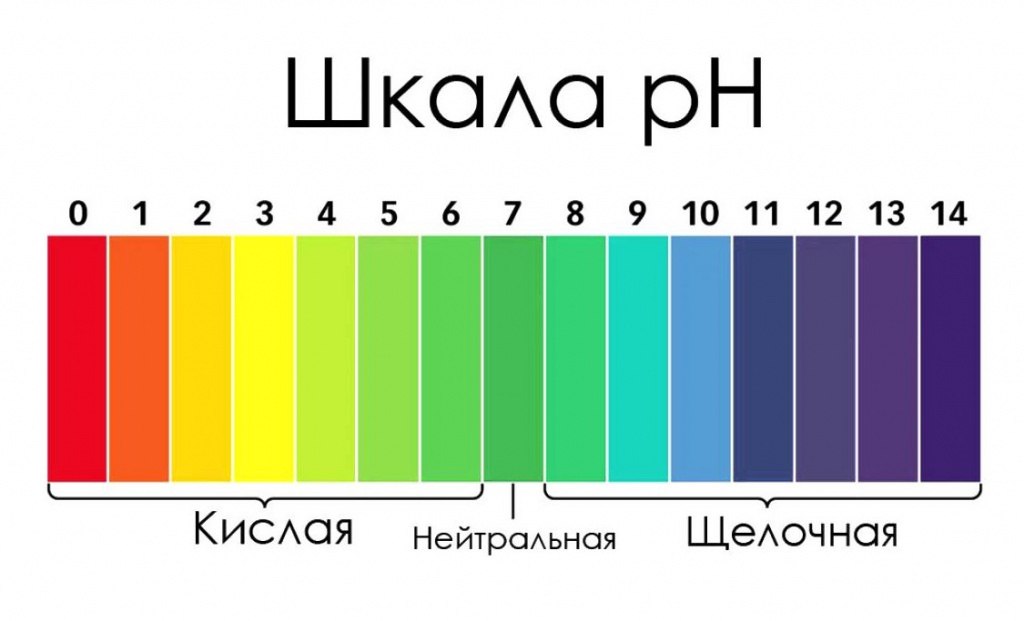
\includegraphics[width=0.6\linewidth]{1.jpg}}
\caption{Шкала pH}
\label{ris1}
\end{figure}


\newpage
\vspace{5cm}
\begin{center}
\textbf{Висновки з виконаної роботи}
\end{center}
Використовуючи рис.\ref{ris1} та дані з таб.\ref{tab2}, можна стверджувати що після проведення електролізу в комірці утворилося кисле середовище, а поза коміркою -- лужне. Що стосується того, що в однорідному електроліті струм менший, то через те що він є нейтральним, без надлишку йонів водню до анода чи катода, а при
неоднорідному електроліті в комірці став надлишок йонів
водню, що створило саме кисле середовище.%, і тим самим швидше більш електронегативний метал із пари електродів почне відновлюватись,


\end{document}